Następująca część pracy obejmuje badanie rozszerzonych możliwości JMetera, czyli pisania w nim testów funkcjonalnych dla aplikacji webowej. W tym rozdziale zostanie opisane środowisko testowe, przykładowe przypadki testowe dla niego oraz rezultaty przeprowadzonej automatyzacji.

\section{Środowisko testowe}
\noindent Cały element badawczy pracy został wykonany przy użyciu następujących elementów:
\begin{itemize}
\item laptopa Lenovo ThinkPad X230, na którym wykonano cały eksperyment;
\item systemu operacyjnego Windows 7 w wersji 64-bitowej;
\item aplikacji webowej napisanej z użyciem konta w WordPress, do której zostały napisane przykładowe testy. Jest to prosta strona internetowa z gotowym wpisem i dwoma odnośnikami do kontaktu oraz do przekierowania na stronę główną; 
\item narzędzia JMeter w wersji 4.0;
\item Selenium WebDriver do pisania skyptów w jmeterowym komponencie BeanShell Sampler;
\item przeglądarki Chrome wersja 69.0.3497.100 do wykonywania skryptów w Selenium;
\item edytora tekstu Notepad++ do pisania pliku z testami w formacie CSV (\textit{comma-separated values}).
\end{itemize}

\begin{figure}[H]
\centering
\captionsetup{justification=centering}
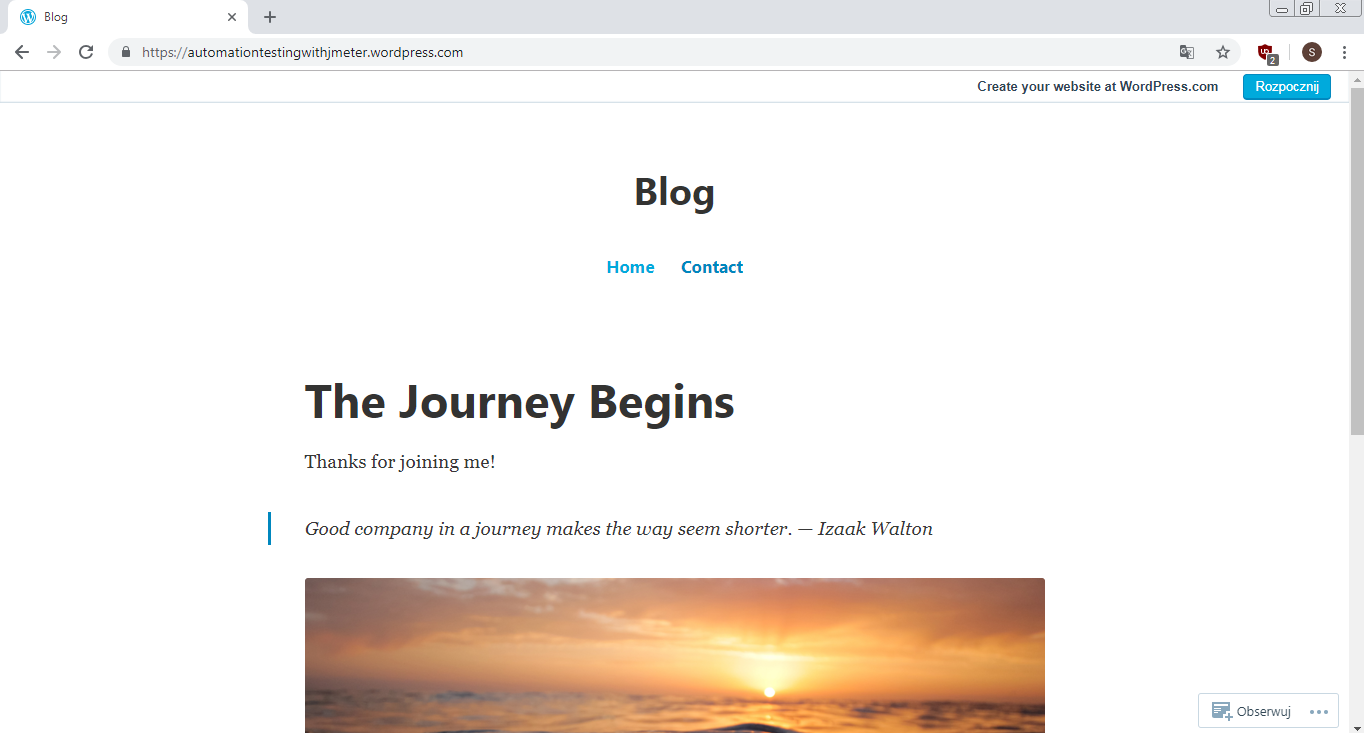
\includegraphics[width=1\textwidth]{Blog.PNG}
\caption[Strona tytułowa bloga]{\label{fig:ham}Strona tytułowa bloga \\ Źródło: opracowanie własne}
\end{figure}


\section{Przedstawienie koncepcji testowania}

Cały pomysł opiera się na wykorzystaniu tzw. bloków testowych jako określonych kroków z parametrem lub parametrami, z których można budować testy napisane w pliku CSV. Bloki te są reprezentowane przez Module Controller. Poniżej zostaną przedstawione te, które zostały zaimplementowane na potrzeby przygotowania testów aplikacji webowej:

\begin{itemize}
\item OPEN\_BROWSER,dummy - otwarcie przeglądarki Chrome i rozszerzenie jej na cały ekran;
\item CLOSE\_BROWSER,dummy - zamknięcie przeglądarki;
\item GO\_TO\_WEBSITE,https://www.google.com/ - przejście do strony podanej jako parametr, tutaj na stronę Google;
\item LOGIN,dummy - logowanie na stronę WordPress;
\item LOGOUT,dummy - wylogowanie z WordPress
\item ADD\_COMMENT,Oto komentarz - dodanie komentarza o treści podanej w parametrze;
\item CHECK\_COMMENT,Oto komentarz - sprawdzenie, czy komentarz o treści 'Oto komentarz' istnieje pod postem
\item MY\_SITE\_PAGE,dummy - przejście po zalogowaniu do zakładki Moja Witryna (w WordPressie); 
\item COMMENT\_OPTION,Accept - zatwierdzenie komentarza w zakładce Komentarze; jest też możliwa opcja Delete, która usuwa istniejący komentarz;
\item MY\_SITE\_PAGE,dummy - przejście do strony Moja Witryna po zalogowaniu się do WordPress;
\item MODIFY\_VISIBILITY,Private - zmiana widoczności bloga na prywatną; możliwość zmiany na Public, czyli każdy może widzieć bloga;
\item CHECK\_VISIBILITY,Private - sprawdzenie na stronie, czy jest ona w trybie prywatnym, czyli czy pojawia się odpowiedni komunikat informujący o tym; 
\item LOGIN\_TO\_SERVER,sylwia:sylwia - zalogowanie się na serwis WordPressa za pomocą użytkownika \textit{sylwia} oraz hasła \textit{sylwia};
\item CHECK\_NEW\_PASSWORD,hasłoDoSprawdzenia - zbadanie, czy hasłoDoSprawdzenia może być zmienione jako nowe dla obecnego użytkownika;
\item ADD\_POST,Post - dodanie postu o tytule Post i sprawdzenie, czy jest on na witrynie;
\item DELETE\_POST,Post - usunięcie postu o tytule Post i sprawdzenie, czy nie ma go na witrynie;
\item ACCEPT\_BUTTON,dummy - naciśnięcie na przycisk na dole ekranu Akceptuj;
\item TAKE\_SCREENSHOT,bug - wykonuje zrzut ekranu w określonym momencie testu i zapisuje do katalogu jako \textit{bug.png}.
\end{itemize}

Warto wspomnieć, że gdy parametr nie jest potrzebny dla danego bloku, wtedy ma on wartość \textit{dummy}).



\begin{figure}[H]
\centering
\captionsetup{justification=centering}
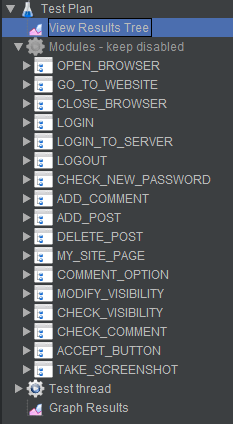
\includegraphics[width=0.7\textwidth]{Modules.PNG}
\caption[Bloki testowe wykorzystywane do pisania testów w ramach pracy]{\label{fig:ham}Bloki testowe wykorzystywane do pisania testów w ramach pracy \\ Źródło: opracowanie własne}
\end{figure}

Sposób, w jaki przedstawiają się komponenty w JMeterze dla naszych testów:
\begin{itemize}
    \item \textit{Test Plan} - zawiera wszystkie niezbędne komponenty;
    \item \textit{View Results Tree} - wyświetla rezultaty kroków wykonywanego testu lub testów;
    \item \textit{Modules - keep disabled} - tam znajdują się bloki testowe składające się głównie z BeanShell Samplera, który wykonuje kawałek kodu napisany z wykorzystaniem Selenium WebDriver;
    \item \textit{Test thread} - w tym miejscu wykonywane są właściwe polecenia:
    \begin{enumerate}
        \item \textit{Configure the CSV file with tests - dummy read for table} - konfiguracja pliku CSV, na początku odczytuje nagłówek, gdzie są zainicjowane zmienne.
        \item \textit{Itearte tests.csv file (While Controller)}, który przechodzi po wspomnianym pliku CSV dopóki nie napotka słowa \textit{END}. W nim wykonuje się wczytywanie kroków z pliku \textit{tests.csv}.
        \item \textit{Configure the CSV file with tests} - ponowna konfiguracja pliku CSV, ale tym razem z testami - przypisanie do wcześniej zainicjowanych w kroku 1. zmiennych odpowiadających im wartości.
        \item \textit{Validate test-case name} - sprawdzenie, czy na początku linii nie występuje symbol \#, który oznacza, że dany test się nie wykona. Jeżeli jest, to wraca się do punktu 2.
        \item \textit{If end of file not reached yet (If Controller)} - gdy warunek, że plik nie napotkał do tej pory słowa \textit{END} jest prawdziwy, to wykonują się dalsze kroki.
        \item \textit{Print in the console the test number and its name} - drukuje w konsoli, na której uruchomiono JMetera, komunikat, który test się wykonuje, czyli numer i jego nazwę.
        \item \textit{===>>> Execute test...} - informacja w JMeterze w nagłówku, który test się teraz wykonuje.
        \item \textit{While current step is not equal to DONE  - test not finished} - pętla działająca do momentu, aż nie pojawi się słowo \textit{DONE}, które oznacza koniec testu.
        \item \textit{Compose step content} - drukuje w konsoli z punktu 6. informację o kroku testowym oraz wartości mu przypisanej.
        \item \textit{If step = STEP} - przypisuje odpowiednie moduły dla podanego kroku (w tym wypadku dla STEP).
        \item \textit{Increment current $\$\{current\}$. step number} - zwiększa numer kroku testowego. 
    \end{enumerate}
\end{itemize}



\begin{figure}[H]
\centering
\captionsetup{justification=centering}
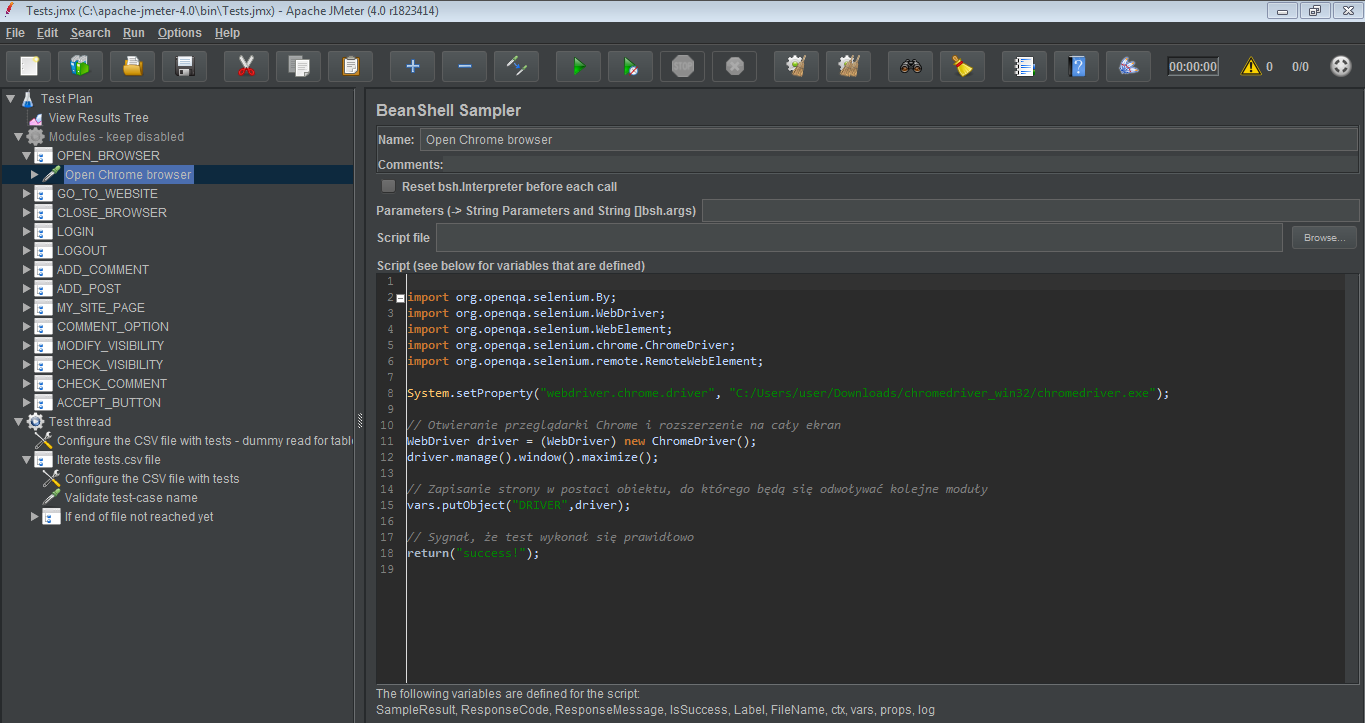
\includegraphics[width=1\textwidth]{Exmpl1.PNG}
\caption[Przykładowy building block OPEN\_BROWSER z pokazanym skryptem wykorzystującym biblioteki Selenium WebDriver]{\label{fig:ham}Przykładowy blok testowy OPEN\_BROWSER z pokazanym skryptem wykorzystującym biblioteki Selenium WebDriver \\ Źródło: opracowanie własne}
\end{figure}

\begin{figure}[H]
\centering
\captionsetup{justification=centering}
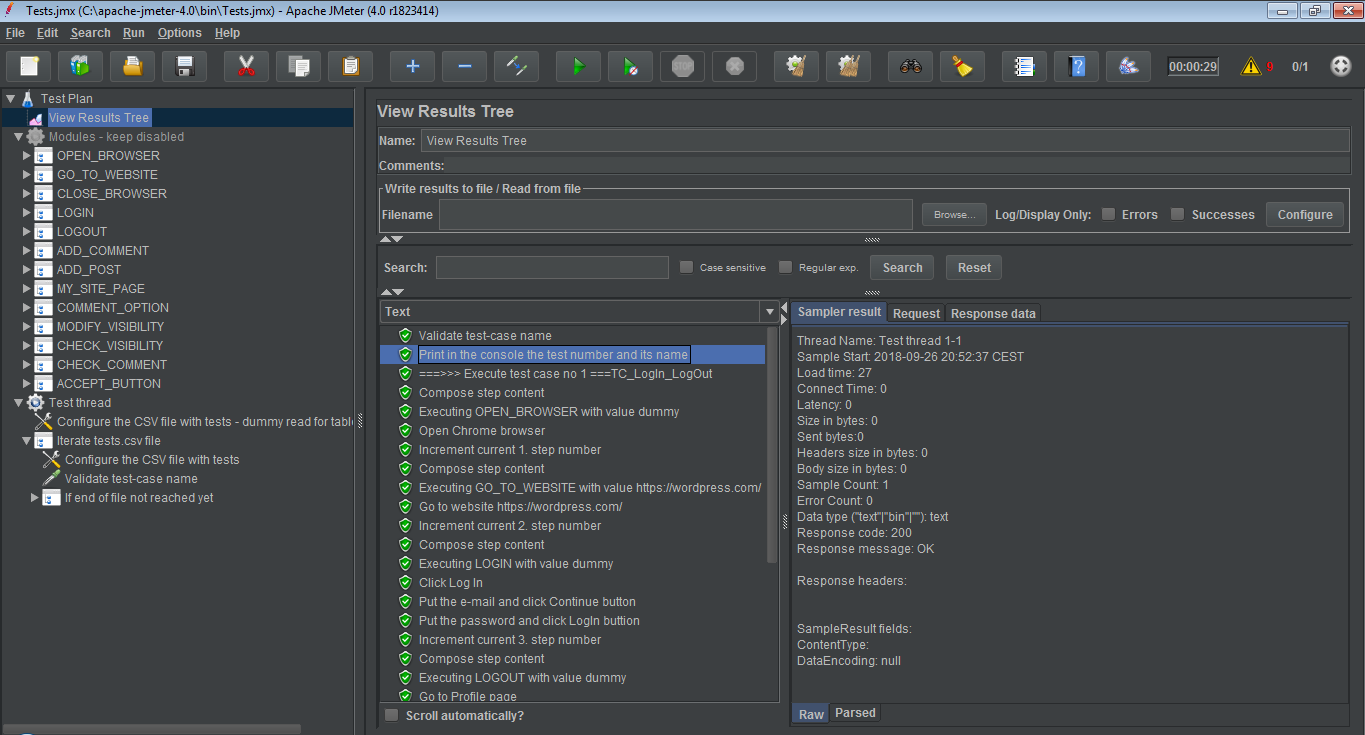
\includegraphics[width=1\textwidth]{Exmpl2.PNG}
\caption[View Results Tree po wykonaniu się pierwszego testu]{\label{fig:ham}View Results Tree po wykonaniu się pierwszego testu \\ Źródło: opracowanie własne}
\end{figure}








